\chapter{System Under Consideration} \label{ch:system}
The following chapter gives a thorough explanation of the system under consideration in this thesis. Firstly, the process of selecting what system to investigate is explained. The system in question is the \textit{SecuritasHome startpaket}\footnotelink{https://www.securitashome.se/product.html/securitashome}{2021-04-14}, which is a home alarm system from Securitas. This starter kit includes multiple hardware components, as well as access to software portals and mobile applications to control the system.

\section{Selection of the system} \label{ch:system:selection}
When starting this project, there were many aspects to consider regarding what system to investigate. The first aspect was \textit{impact}. If the security was compromised what consequences would that have? Hacking a doorbell might lead to annoyances, while a smart pacemaker could have lethal consequences. Smart home alarm systems have the potential for a huge impact. Gaining physical access to a house without any alarm system is not difficult. It is as easy as breaking a window. People, therefore, rely on alarm systems to deter criminals and to immediately notify security personnel of a breach. The worst consequence of a cybersecurity vulnerability in such a system would be to completely disarm an armed system, without authorization, thereby granting easy access to a property without, potentially, getting caught.

Another aspect to consider is \textit{vulnerability}. What is the likelihood to find a vulnerability in the system? There are several things to consider to answer that question. One is the reputation of the manufacturer. Are there many previously reported vulnerabilities on their systems? Are they known for caring about security and producing secure products? Another is how complex the system is. Does it have many features and components? How large is the system's attack surface? Smart home alarm systems have become increasingly complex, leading to a relatively large attack surface.

Due to the reasons mentioned above, smart home alarm systems were deemed an excellent target for this thesis. The last thing to consider was therefore how feasible it is to procure the system, and importantly if one has the legal rights to security test it. In Sweden, the two largest companies in the industry are \textit{Verisure}\footnotelink{https://www.verisure.se/}{2021-04-15} and \textit{Sector Alarm}\footnotelink{https://www.sectoralarm.se/}{2021-04-15}. Systems from these companies were considered in the early phase of the project and both were contacted through their customer support to assess the feasibility to procure the system and if it would be legal to do a security evaluation. Both companies, unfortunately, failed in this criteria. In Sweden, the law regarding cybersecurity evaluations, in simplified terms, says you have to have the owner's permission to security test a system (\todo: source). Both companies stated firmly that they would continue to own the physical system and require that their technicians install the system on the premise. Both seemed unwilling to let you buy out the system, and were therefore ruled out. In the case of SecuritasHome, on the other hand, you own the system and pay a monthly fee to access their software platform and security personnel in case of a breach. This, along with the aspects described above, made the SecuritasHome system a good target for security analysis.

\section{The companies behind the system} \label{ch:system:companies}
This section covers the structure of the three major companies behind the SecuritasHome Home Alarm System.

While the system is sold and branded by SecuritasHome, they actually have little to do with the actual hardware and software components of the platform, see figure \ref{fig:company-structure}. The hardware, related firmware, and proprietary radio wave protocol for communication between the components are manufactured and produced by a Taiwanese company called \textit{Climax Technology}\footnotelink{https://www.climax.com.tw/}{2021-04-01}. They are a major manufacturer of wireless home security systems and produce hardware for home consumer security. They design everything from smart home alarm systems, and smart garage door openers, to smart medical accessories for seniors. The software, like the web portal and mobile applications as well as some additional firmware, is developed by an American company called \textit{Alarm.com}\footnotelink{https://alarm.com/}{2021-04-01}. They are strictly a B2B (business to business) company, meaning they do not sell or advertise their product directly to the end consumer. Instead, they outsource the sale and advertisement of the system to partner companies, one of them being SecuritasHome. SecuritasHome merely sells, advertise, and put their brand on the product. Their main contribution to the system is in terms of real-time response to an alarm, customer service, connection to an alarm-central, and sending security personnel to respond to an active alarm breach. Consequently, when considering the cybersecurity of the system, SecuritasHome is not highly relevant. The two relevant parties are \textit{Alarm.com} and, considering the focus of this thesis, especially \textit{Climax Technology}.
\begin{figure}[!ht]
    \centering
    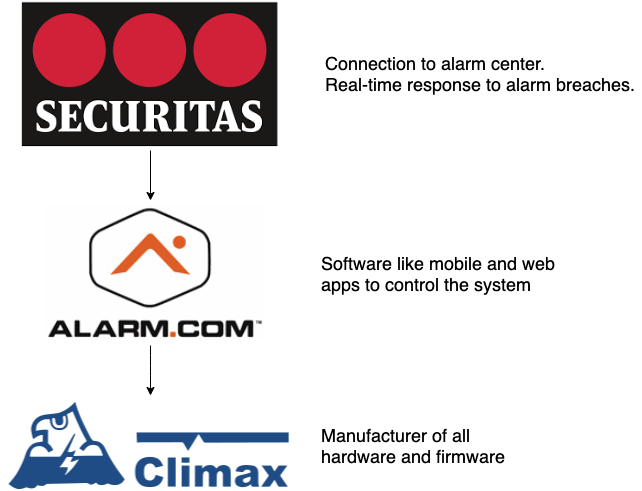
\includegraphics[width=0.7\textwidth]{images/3-system/company-structure.png}
    \caption{The companies behind the system.}
    \label{fig:company-structure}
\end{figure}

\section{Components and Software} \label{ch:system:components}
This section describes all the components and software of the system. Initially, all hardware components are described and their functionality. Lastly, all software components of the system are described. Note that the system supports many additional hardware components. The ones outlined below are only the ones part of the starter kit.

\subsection{Hardware components} \label{ch:system:hardware}
The SecuritasHome starter kit contains five hardware components, see figure \ref{fig:hardware-components}. These are described below. Note that the system supports many additional components, like smart locks for example. However, only the components included in the starter kit are covered in this thesis.
\begin{figure}[!ht]
    \centering
    \begin{subfigure}[t]{0.33\textwidth}
        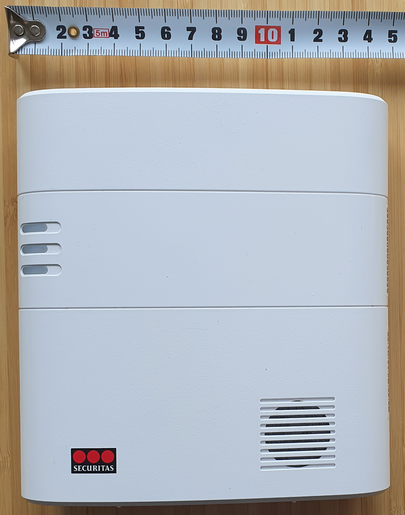
\includegraphics[height=2.15in]{images/3-system/main-panel.png}
        \caption{Main Panel}
        \label{fig:main-panel}
    \end{subfigure}%
    ~
    \begin{subfigure}[t]{0.33\textwidth}
        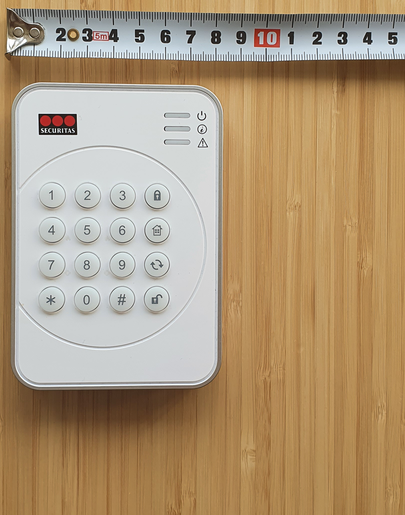
\includegraphics[height=2.15in]{images/3-system/keypad.png}
        \caption{Remote Keypad}
        \label{fig:remote-keypad}
    \end{subfigure}%
    ~
    \begin{subfigure}[t]{0.33\textwidth}
        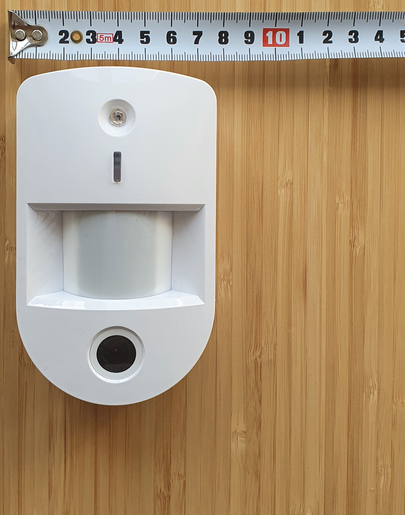
\includegraphics[height=2.15in]{images/3-system/camera.png}
        \caption{Motion Detection Camera}
        \label{fig:motion-camera}
    \end{subfigure}
    
    \begin{subfigure}[t]{0.33\textwidth}
        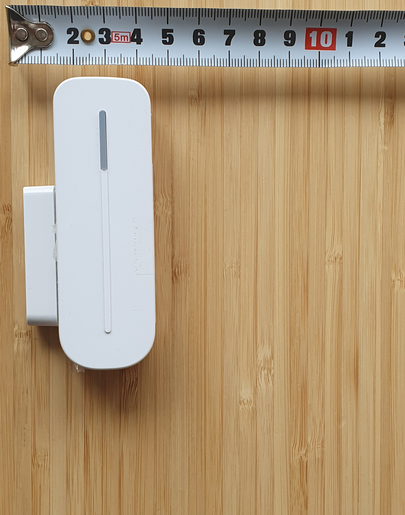
\includegraphics[height=2.15in]{images/3-system/door-contact.png}
        \caption{Door Contact Sensor}
        \label{fig:door-contact}
    \end{subfigure}%
    ~
    \begin{subfigure}[t]{0.33\textwidth}
        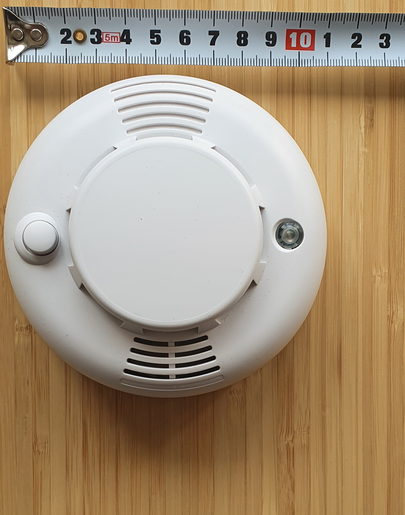
\includegraphics[height=2.15in]{images/3-system/smoke-detector.png}
        \caption{Smoke Detector}
        \label{fig:smoke-detector}
    \end{subfigure}
    \caption{The hardware components of the system.}
    \label{fig:hardware-components}
\end{figure}
\subsubsection{Main Panel}
\textbf{Model number:} HSGW-G8-3G/LTE-ZW-F1 433/868 \\
\textbf{FCCID:} GX9HSGWF1919 \\
The main panel, see figure \ref{fig:main-panel}, is the \textit{"brains"} of the system so to speak. It handles communication with all other hardware devices as well as external servers. Through radio wave communication it communicates to all the other hardware peripherals of the system. It uses 3G telecommunication to communicate with the external servers. It also has an Ethernet port to connect to the local network, the purpose of which is unclear. The panel also has a tamper sensor, which triggers if the plastic back panel is taken off.

\subsubsection{Remote Keypad}
\textbf{Model number:} KPT-23-EL-F1 \\ % could also be KPT-23N-EL-F1, not sure
\textbf{FCCID:} GX9KPF1 \\ % This says KPF, not KPT, but it looks the same?
The remote keypad is a 16 button keypad used to arm and disarm the system using a personal 4 digit pin. See figure \ref{fig:remote-keypad}. This device communicates with the main panel over radio wave communication.

\subsubsection{Motion Detection Camera}
\textbf{Model number:} VST-862-F1 \\
\textbf{FCCID:} GX9862 \\
This device, see figure \ref{fig:motion-camera}, features an infra-red sensor to detect motion, and a camera to survey the location. When triggered the device takes two pictures which are sent to the main panel. It is not a surveillance camera, meaning it does not continuously take pictures. The camera is only active when motion is detected and the alarm is triggered, presumably to save power. The camera also features a tamper sensor, which triggers if it is not properly attached against the wall.

\subsubsection{Door Contact Sensor}
\textbf{Model number:} DC-23-F1 \\
\textbf{FCCID:} GX9DC23 \\
This device, see figure \ref{fig:door-contact}, senses when a door or window is opened. A small external magnet is placed on the door/window close to the device. When these are separated the device is triggered and communicates with the main panel over radio wave communication. Like the camera, it also features a tamper sensor, which triggers if it is not properly attached against the wall.

\subsubsection{Smoke Detector}
\textbf{Model number:} SD-8EL \\
\textbf{FCCID:} GX9SD8ELF1919 \\
This device is a smoke detector, see figure \ref{fig:smoke-detector}. It communicates with the main panel over radio waves and also includes a siren that triggers when it detects smoke.

\subsubsection{Additional peripherals}
The system supports many additional devices not included in the \textit{SecuritasHome startpaket}. These include for example water leakage sensors\footnotelink{https://www.securitashome.se/product.html/vattendetektor-2}{2021-05-25}, temperature sensors\footnotelink{https://www.securitashome.se/product.html/temperatursensor}{2021-05-25}, IP cameras over both WiFi\footnotelink{https://www.securitashome.se/product.html/ip-kamera-inne-wifi}{2021-05-25} and PoE\footnotelink{https://www.securitashome.se/product.html/ip-kamera-ute}{2021-05-25}, and smart locks.

Additionally, the system supports controlling devices over the Z-Wave protocol\footnotelink{https://en.wikipedia.org/wiki/Z-Wave}{2021-05-25}. This allows a whole plethora of devices to be connected to and controlled by the system such as smart light bulbs for example. This include devices from completely different manufacturers.

Note that the devices covered in this section are delimited from this project and thus not covered in the report.

\subsection{Software} \label{ch:system:software}
This section details the three software entry points from where the user can control the alarm and view its state.

\subsubsection{Web portal}
The web portal is a web page created by the American company \textit{Alarm.com}, see figure \ref{fig:company-structure}, hosted at \url{https://www.alarm.com/web/system/}. From the landing page, see figure \ref{fig:web-landing-page}, the user can see the following:
\begin{itemize}
    \item If the system has any issues. This can be seen in the \textit{System OK} box in figure \ref{fig:web-landing-page}.
    \item The state of each sensor of the system, like the door contact sensor (see figure \ref{fig:door-contact}).
    \item The arm/disarm state of the system.
    \item The latest photograph taken by the motion detection camera (see figure \ref{fig:motion-camera}).
    \item Request a photo from the camera to be taken either directly or on the next detected movement.
\end{itemize}
Crucially, from the landing page, the user can also easily arm or disarm the system, see figure \ref{fig:web-arming}. Beyond this, the user can also see a list of recent activity in the system, change the user's personal four-digit pin codes, and create new users.
\begin{figure}[!ht]
    \centering
    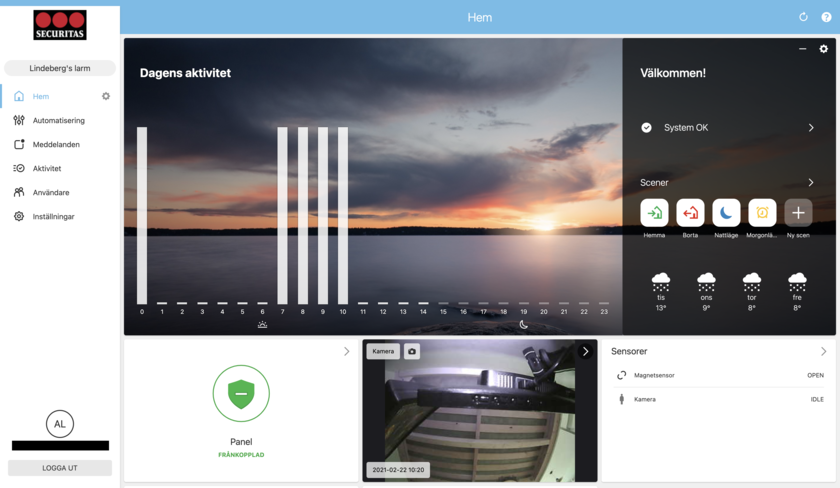
\includegraphics[width=\textwidth]{images/3-system/landing-page-web.png}
    \caption{The web portal landing page.}
    \label{fig:web-landing-page}
\end{figure}
\begin{figure}[!ht]
    \centering
    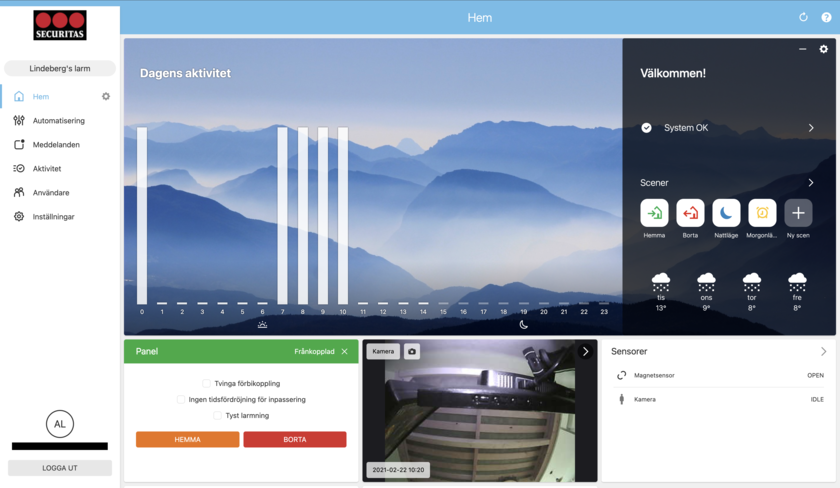
\includegraphics[width=\textwidth]{images/3-system/arming-web.png}
    \caption{Arming the alarm from the web portal.}
    \label{fig:web-arming}
\end{figure}

\subsubsection{Mobile application}
The system can also be controlled and administrated via a mobile application (see figure \ref{fig:mobile-application}), free to download via the \textit{Google Play Store}, called \textit{Securitas Connect}\footnotelink{https://play.google.com/store/apps/details?id=com.alarm.alarmmobile.android.securitas}{2021-03-30}, and from the \textit{App Store}, for iOS devices, under the same name\footnotelink{https://apps.apple.com/se/app/securitas-connect/id1111700213}{2021-04-14}. As explained previously, while the application is branded by Securitas, it is created and developed by \textit{Alarm.com}. The interface very closely resembles the web portal, see figure \ref{fig:mobile-landing-page}, and offers identical functionality. The only additional feature is real-time notifications of any changes in the system, done via push notifications to your mobile device, as shown in figure \ref{fig:mobile-notification}. This could be for example the door contact sensor triggering, the main panel losing external power due to a power outage, or the alarm being armed/disarmed.
\begin{figure}[!ht]
    \centering
    \begin{subfigure}[t]{0.5\textwidth}
        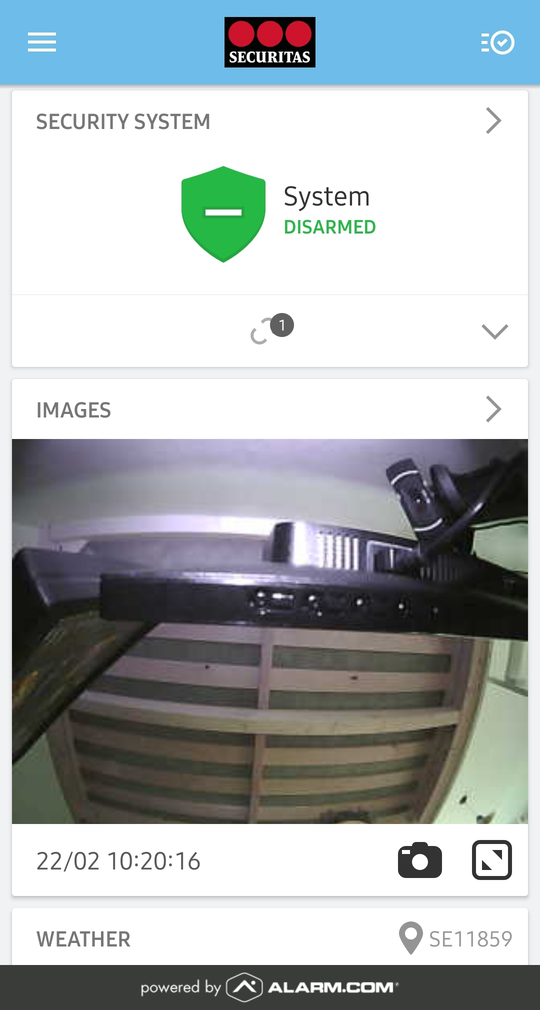
\includegraphics[height=4.8in]{images/3-system/mobile-landing-page.png}
        \caption{The mobile app's landing page.}
        \label{fig:mobile-landing-page}
    \end{subfigure}%
    ~
    \begin{subfigure}[t]{0.5\textwidth}
        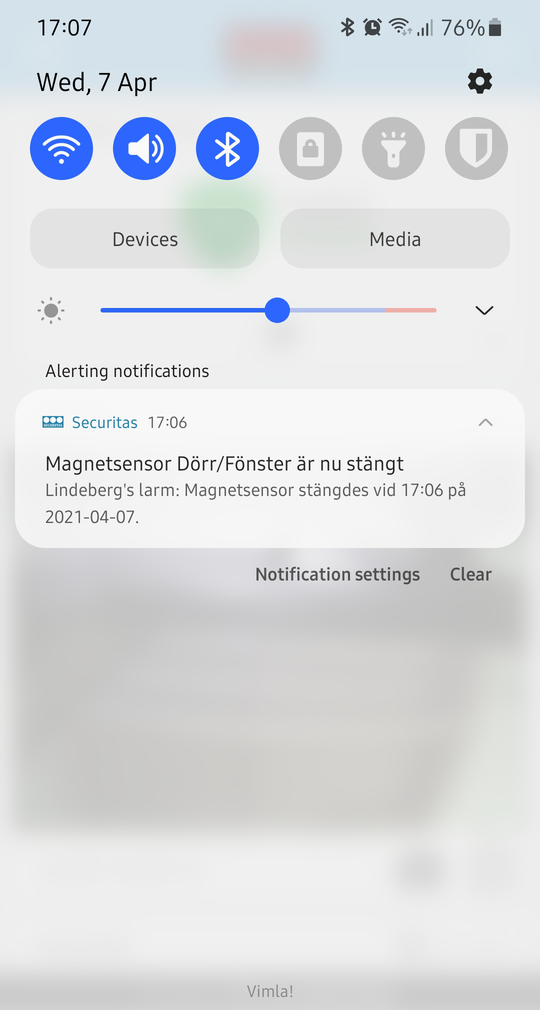
\includegraphics[height=4.8in]{images/3-system/mobile-notification.png}
        \caption{A notification triggered by the door contact sensor.}
        \label{fig:mobile-notification}
    \end{subfigure}
    \caption{The Securitas Connect mobile app.}
    \label{fig:mobile-application}
\end{figure}

\subsubsection{Local web admin page}
Beyond the two applications created by \textit{Alarm.com} described above, the main panel (see figure \ref{fig:main-panel}) hosts a web server on the local network. This feature is undocumented and is presumably not meant to be used or found by the regular, non-tech-savvy consumer. The page is not hosted on any domain name, as far as the author is aware, and instead has to be accessed directly via the main panel's local IP address on port 80. The landing page of this web server, see figure \ref{fig:local-landing-page}, is quite simple and shows some basic information about the system such as the MAC address, IMEI number of the cellular communication, etc. Beyond that, the site only has two actions the user can do. One is to perform a "\textit{Phone Test}", to presumably test the connection to the mobile 3G network, and the other is a "\textit{Network Scan}". Once the network scan has completed, the page shows a list of all reachable telecommunication towers, see figure \ref{fig:local-network-scan}.
\begin{figure}[!ht]
    \centering
    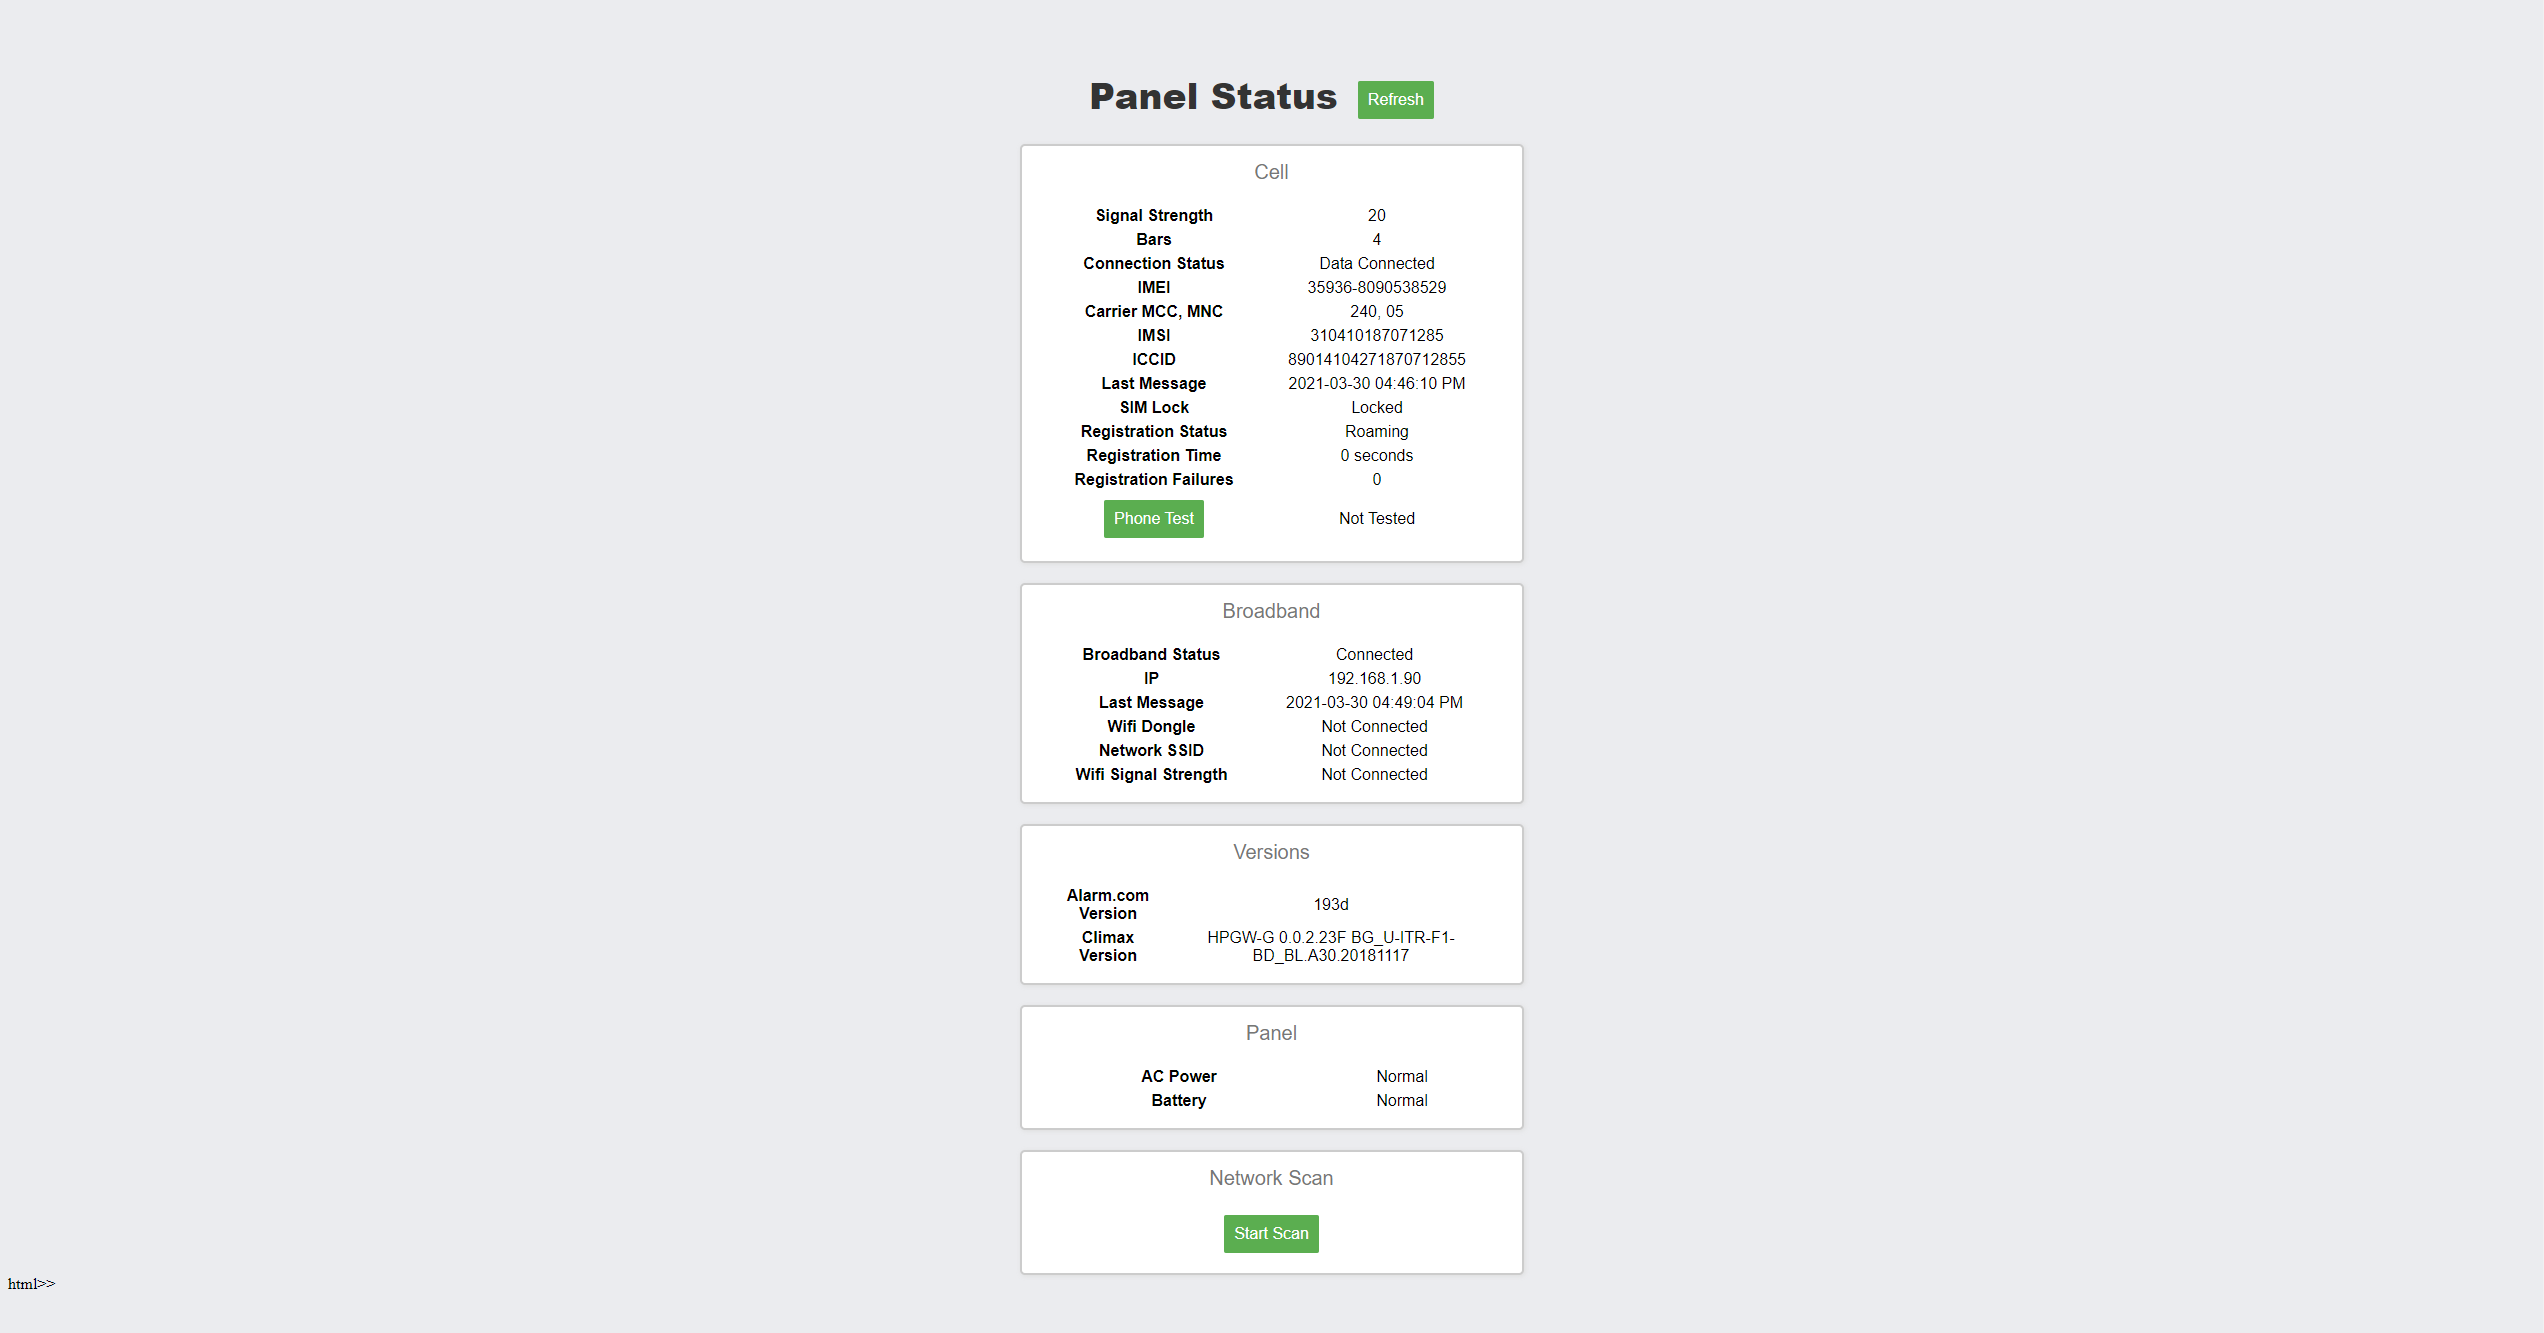
\includegraphics[width=\textwidth]{images/3-system/local-landing-page.png}
    \caption{The local web server's landing page.}
    \label{fig:local-landing-page}
\end{figure}
\begin{figure}[!ht]
    \centering
    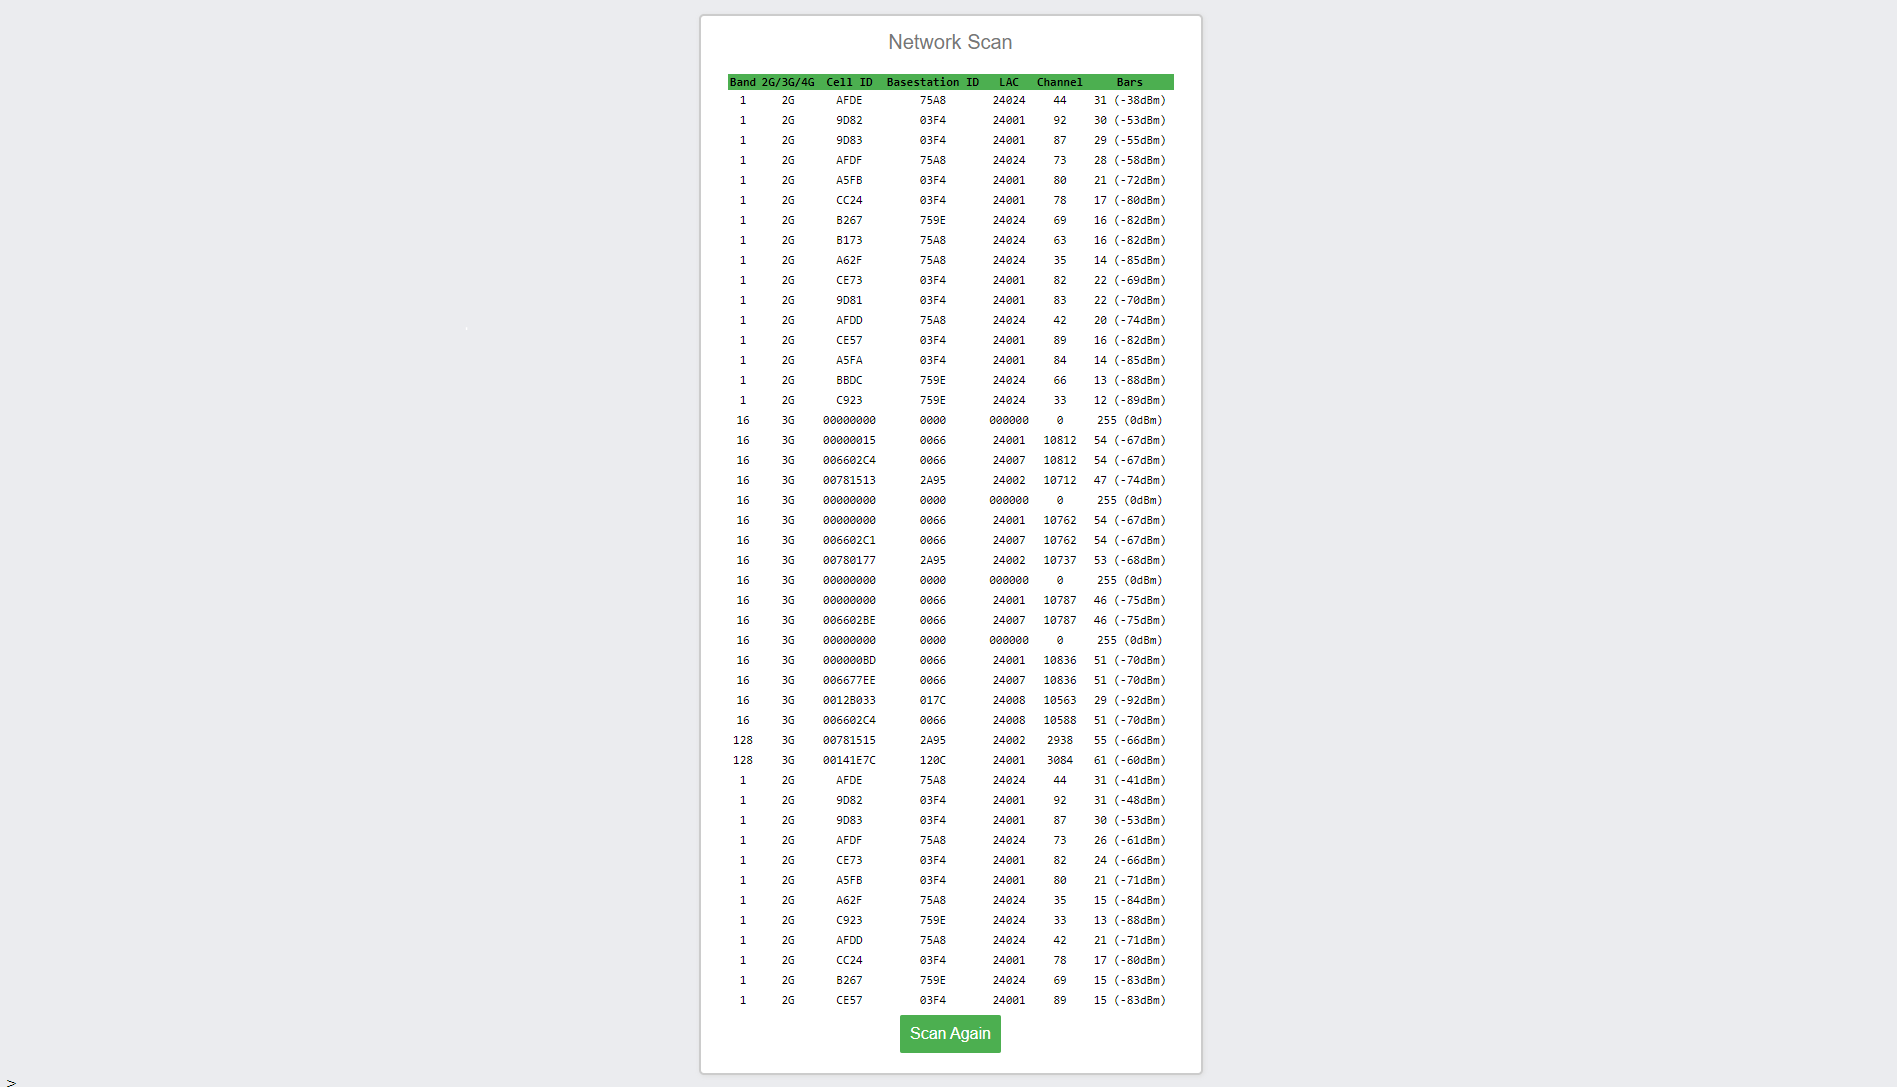
\includegraphics[width=\textwidth]{images/3-system/local-network-scan.png}
    \caption{A mobile network scan from the local web server.}
    \label{fig:local-network-scan}
\end{figure}
\begin{figure}[!ht]
    \centering
    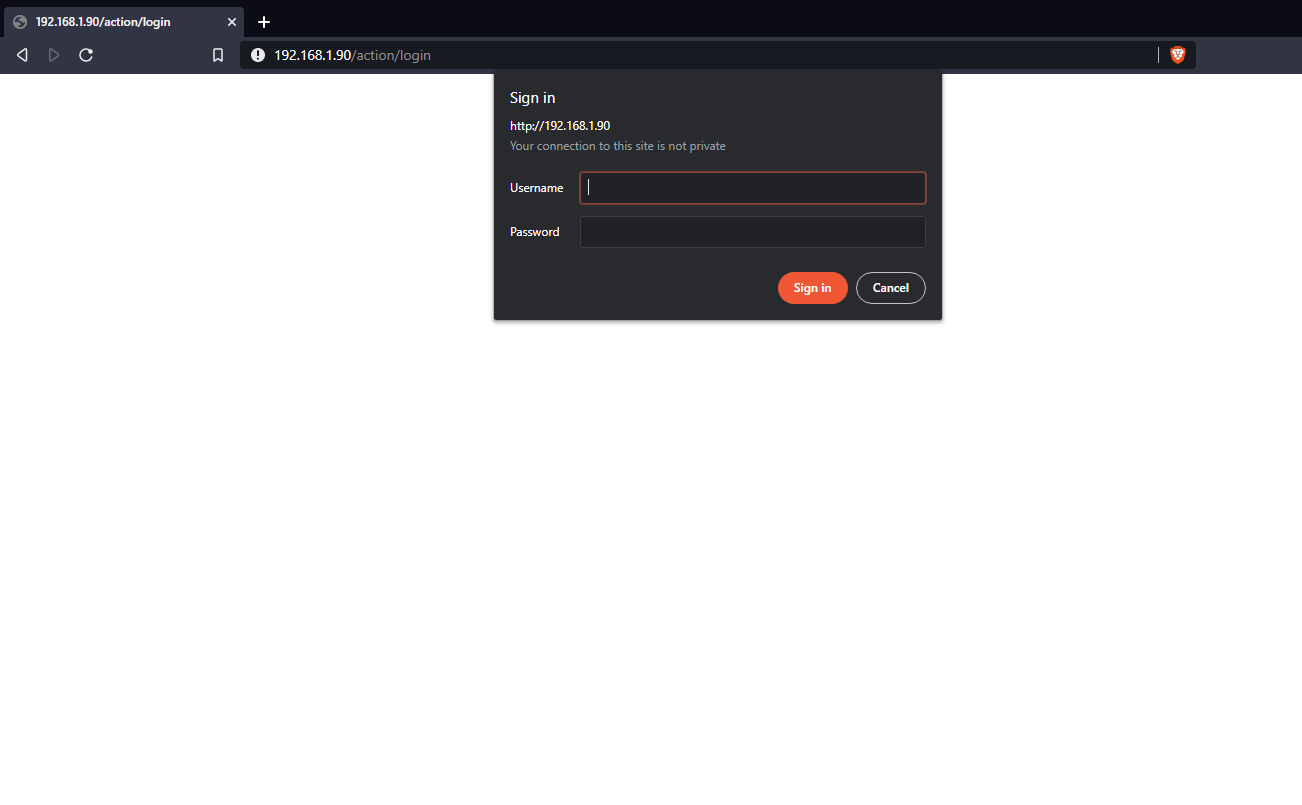
\includegraphics[width=\textwidth]{images/3-system/local-login-page.png}
    \caption{The local web server's HTTP Basic Auth login page.}
    \label{fig:local-login-page}
\end{figure}
\begin{figure}[!ht]
    \centering
    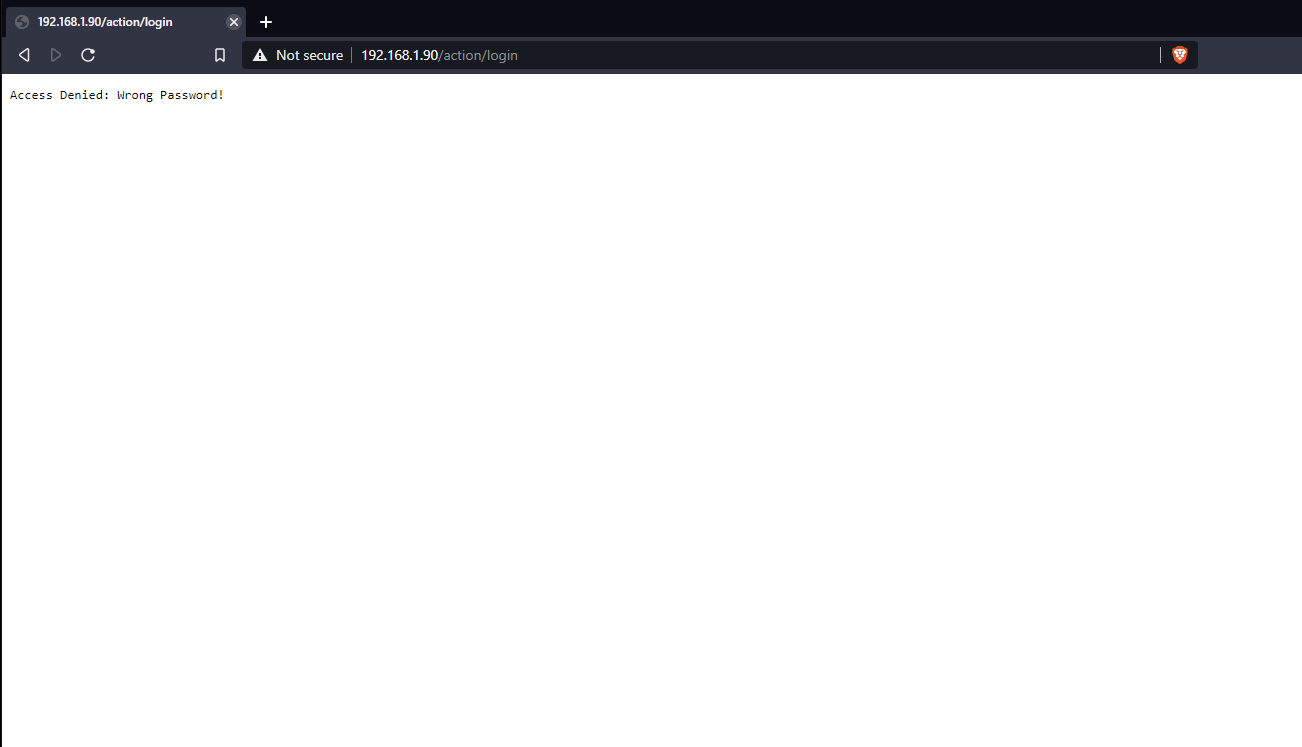
\includegraphics[width=\textwidth]{images/3-system/local-login-denied.png}
    \caption{A failed login attempt on the local web server.}
    \label{fig:local-login-denied}
\end{figure}
Additionally, the web page features an undocumented login page on the path \texttt{/action/login}, see figure \ref{fig:local-login-page}. This page lets the user authenticate using \textit{HTTP Basic auth}. The credentials here are not tied to the user's account on the aforementioned web portal or mobile applications. Presumably, this is purely meant as a backdoor for the manufacturer for debugging purposes, and not meant to be used by the user of the system. If wrong credentials are entered the user is presented with a static message, saying they have the wrong password (see figure \ref{fig:local-login-denied}), providing zero additional functionality.
